% ============================================================
% CHAPITRE II — ÉTAT DE L'ART
% ============================================================
\chapter{ARCHITECTURE ET CONCEPTION}

\section*{Introduction}
\addcontentsline{toc}{section}{Introduction}

Ce chapitre présente l’architecture globale du système ainsi que les principaux choix de conception adoptés afin de répondre aux exigences fonctionnelles et non fonctionnelles du projet. Dans un contexte où le système intègre des objets connectés, des modules d’intelligence artificielle et des interfaces multi-utilisateurs, la définition d’une architecture claire et structurée constitue un enjeu essentiel pour garantir la cohérence, la maintenabilité et l’évolutivité de la solution.

Afin de maîtriser cette complexité, une approche architecturale en couches a été adoptée. Cette décomposition permet d’isoler les responsabilités de chaque composant du système, en distinguant les fonctions liées à l’acquisition des données, à la communication, au traitement centralisé et à l’interaction utilisateur. Chaque couche est conçue de manière indépendante tout en restant fortement interconnectée avec les autres, assurant ainsi une bonne interopérabilité et une meilleure robustesse globale.

Dans la suite de ce chapitre, l’architecture est analysée selon une décomposition en modules fonctionnels complémentaires. Le module IoT présente les équipements de la serre ainsi que les dispositifs embarqués assurant la collecte et le contrôle des données. Le module d’intelligence artificielle décrit les architectures mises en œuvre pour les modèles développés ainsi que les approches méthodologiques adoptées. Le module backend et communication détaille les mécanismes d’orchestration et d’échange des données entre les différents composants. Enfin, le module des interfaces utilisateur expose les environnements de supervision et d’interaction destinés aux différents profils d’utilisateurs.

Cette organisation progressive permet d’assurer une compréhension claire et structurée de l’ensemble de l’architecture du système.
\newpage
% ============================================================
\section{Architecture Globale}
\label{sec:glob}

\subsection{Modèle de référence IoT à 4 couches}
L’architecture du \textit{HydroNova} repose sur un principe fondamental de séparation des responsabilités. Inspirée des modèles de référence de l’Internet des Objets (IoT), cette architecture organise le système en plusieurs couches fonctionnelles indépendantes mais interconnectées. Une telle structuration permet d’assurer une meilleure évolutivité, une maintenance simplifiée ainsi qu’une communication fluide entre les différents composants matériels et logiciels du système.

Le choix d’une architecture IoT en quatre couches répond également aux contraintes spécifiques du contexte agricole intelligent, notamment la nécessité d’un traitement local rapide, la transmission fiable des données, la supervision centralisée et l’accès distant aux services de la plateforme.

Le modèle retenu se compose des couches suivantes :

\begin{itemize}
	
	\item \textbf{Couche 1: Objets et Composants IoT :}  
	Cette couche constitue le niveau physique du système et regroupe l’ensemble des équipements déployés dans la serre. Elle assure la collecte des données environnementales à travers les capteurs, le contrôle des équipements via les actionneurs ainsi que l’exécution locale des traitements embarqués. Elle intègre également un module d’intelligence artificielle embarquée permettant l’analyse locale des images afin de détecter les anomalies ou maladies des cultures. Cette approche réduit la dépendance au cloud, diminue la latence et garantit la continuité du fonctionnement même en cas de perte de connexion réseau.
	
	\item \textbf{Couche 2: Communication et Transport des Données :}  
	Cette couche assure la connectivité entre les dispositifs IoT, la plateforme centrale et les interfaces utilisateur. Son rôle principal consiste à garantir l’échange fiable, sécurisé et bidirectionnel des données et des commandes entre les différentes composantes du système. Elle prend en charge la transmission des données de télémétrie, des alertes intelligentes ainsi que des commandes de contrôle envoyées vers les équipements de la serre. Cette séparation de la couche réseau améliore l’interopérabilité entre les dispositifs et facilite l’intégration future de nouveaux équipements ou services.
	
	\item \textbf{Couche 3: Cloud et Backend :}  
	Cette couche représente le centre de traitement et d’orchestration du système. Elle assure la persistance des données, l’exécution de la logique métier, l’analyse des informations collectées ainsi que la gestion des utilisateurs et des droits d’accès. Elle centralise également les services intelligents de la plateforme et coordonne les interactions entre les objets connectés et les applications clientes. Cette couche permet d’exploiter les données historiques afin de générer des analyses, des alertes et des recommandations destinées à l’aide à la décision agricole.
	
	\item \textbf{Couche 4: Présentation :}  
	Cette couche correspond aux interfaces de communication entre le système et les utilisateurs finaux. Elle fournit des outils de visualisation, de supervision et de contrôle permettant de consulter l’état de la serre, suivre les données en temps réel et interagir avec les différents services disponibles. Elle comprend une application mobile destinée aux agriculteurs et aux visiteurs ainsi qu’une plateforme web dédiée aux administrateurs et aux agents techniques. Cette couche facilite le pilotage à distance et améliore l’accessibilité globale du système.
	
\end{itemize}

L’adoption de cette architecture en couches permet ainsi de garantir une meilleure modularité du système, une séparation claire des responsabilités ainsi qu’une plus grande flexibilité pour l’évolution future de la plateforme.

\begin{figure}[!htbp]
	\centering
	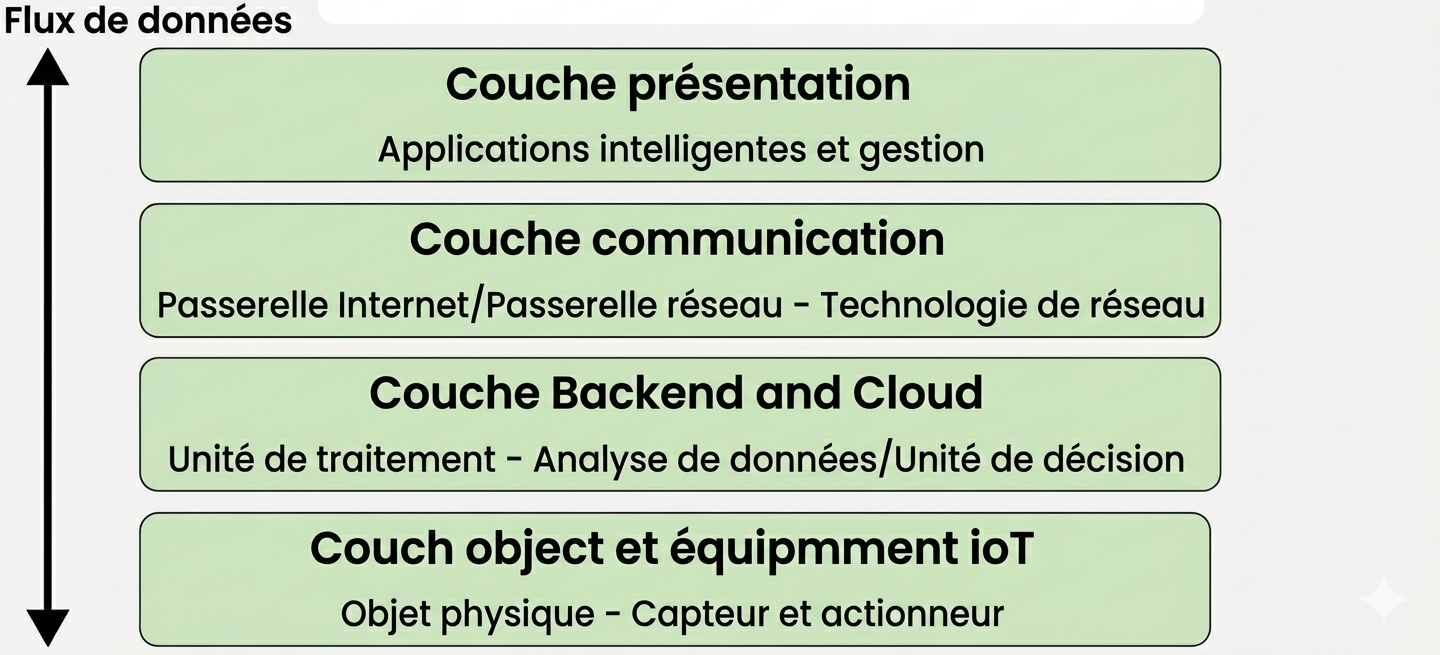
\includegraphics[width=0.7\linewidth]{public/4couche}
	\caption{Modèle IoT en 4 couches}
	\label{fig:4couche}
\end{figure}


\subsection{Flux de données global: bout en bout}
La figure \ref{fig:archi_globale} illustre cette architecture en mettant en évidence l’organisation en couches ainsi que les flux de communication entre les différents niveaux du système. Elle permet de visualiser clairement la séparation des responsabilités et le rôle de chaque composant dans le fonctionnement global de la solution.
\begin{figure}[!htbp]
	\centering
	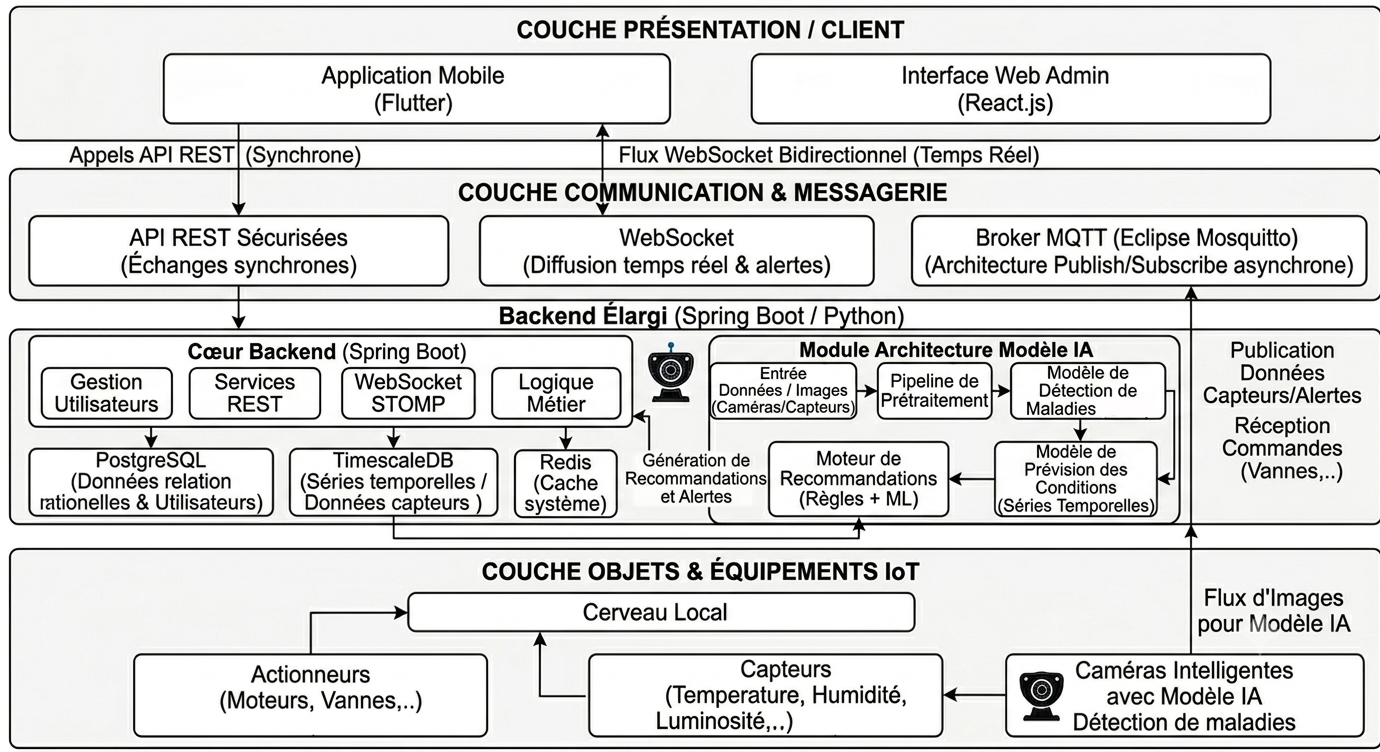
\includegraphics[width=0.95\linewidth]{public/glob.png}
	\caption{Architecture globale du système en quatre couches fonctionnelles}
	\label{fig:archi_globale}
\end{figure}


\newpage

% ============================================================
\section{Architecture Détaillée}
\label{sec:Architecture Détaillée}
% La section IA a été déplacée dans le Chapitre IV (chapitre_ia.tex)
\subsection{Module IoT et Système Embarqué}
%━━━━━━━━━━━━━━━━━━━━━━━━━━━━━━━━━━━━━━━━━━━━━━━━━━━━━━━━━━
\subsubsection{Architecture du module IoT}
L'un des principes directeurs de notre conception est l'\textbf{indépendance vis-à-vis du matériel} : l'architecture du module IoT n'est liée à aucun type de contrôleur particulier. Elle a été pensée comme un cadre générique et extensible, capable d'accueillir n'importe quelle unité de calcul embarquée (Raspberry Pi, BeagleBone, contrôleur industriel, etc.) dès lors que celle-ci respecte le contrat de communication défini par la plateforme. Pour le prototype présenté dans ce projet, le contrôleur retenu se compose d'un \textbf{Raspberry Pi 4} jouant le rôle d'unité Edge, complété par une carte \textbf{Arduino Uno} dédiée à la gestion bas niveau des entrées/sorties matérielles. Ce choix illustre une instanciation possible de l'architecture, sans en constituer une contrainte structurelle.

Cette indépendance s'étend au-delà du seul contrôleur : \textbf{capteurs et actionneurs sont eux aussi des composants extensibles}. Le principe fondateur est qu'à chaque composant physique présent dans la serre correspond une entité dans le backend. Un capteur de température installé sur l'Arduino, une pompe pilotée par un relais, un moteur pas à pas: chacun de ces éléments matériels dispose d'une représentation dans le modèle de données du serveur, portant ses caractéristiques (unité de mesure, commandes supportées, topics de communication). L'intégration d'un nouveau composant physique se résume donc à le déclarer dans ce référentiel commun, sans aucune refonte structurelle ni du micrologiciel ni du backend. C'est cette correspondance biunivoque entre le monde physique et le modèle logiciel qui garantit la compatibilité permanente entre les deux couches et qui permet à l'ensemble du système d'évoluer de façon cohérente.
\subsubsection*{Architecture matérielle de la serre}

La figure~\ref{fig:archi_iot} illustre l’architecture globale du système embarqué de la serre. Elle met en évidence l’organisation des différents composants matériels, notamment les capteurs et les actionneurs, ainsi que leur connexion à la carte Arduino. On y observe également la liaison de communication série assurant l’échange de données entre l’Arduino et le Raspberry Pi 4, qui joue le rôle de passerelle intelligente vers le système de traitement.

\begin{figure}[!htbp]
	\centering
	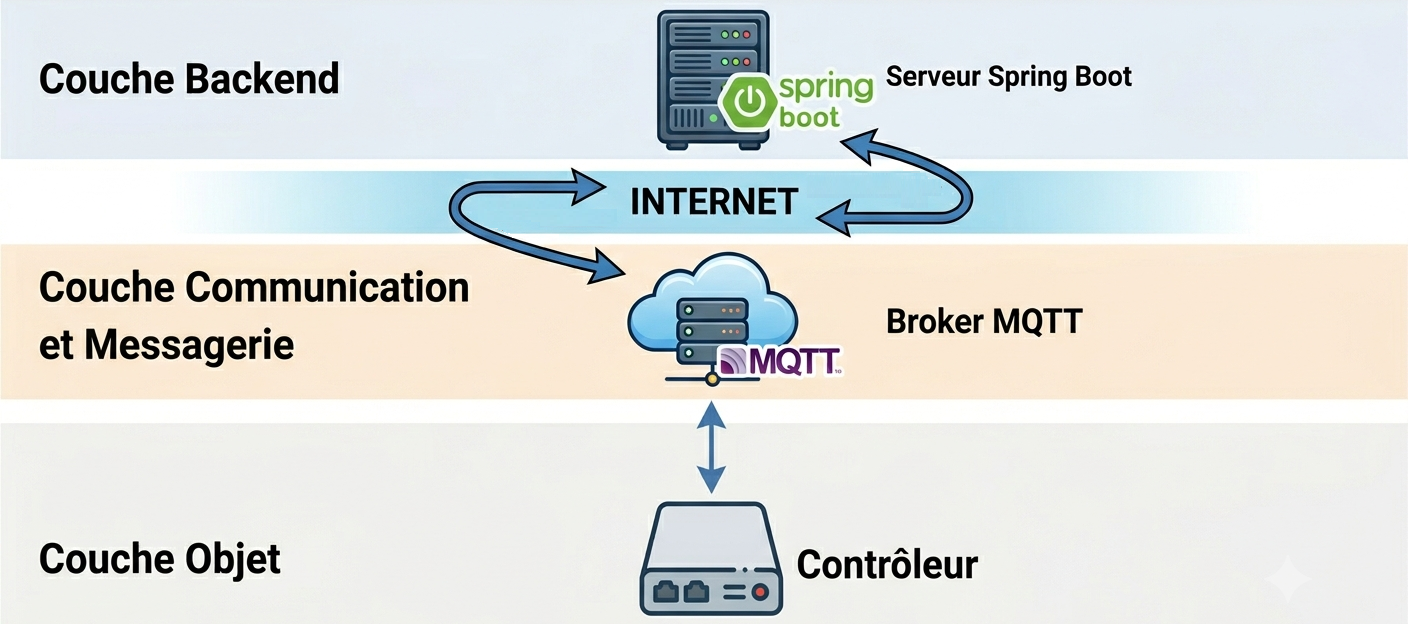
\includegraphics[width=0.8\linewidth]{public/archi_IOTF}
	\caption{Architecture globale du système IoT de la serre intelligente}
	\label{fig:archi_iot}
\end{figure}

Afin de détailler davantage l’implémentation physique du système, la figure~\ref{fig:cablage} présente le schéma de câblage des capteurs et des actionneurs connectés au contrôleur principal. Elle permet de visualiser précisément les connexions électriques et la répartition des composants au sein de la serre.

\begin{figure}[!htbp]
	\centering
	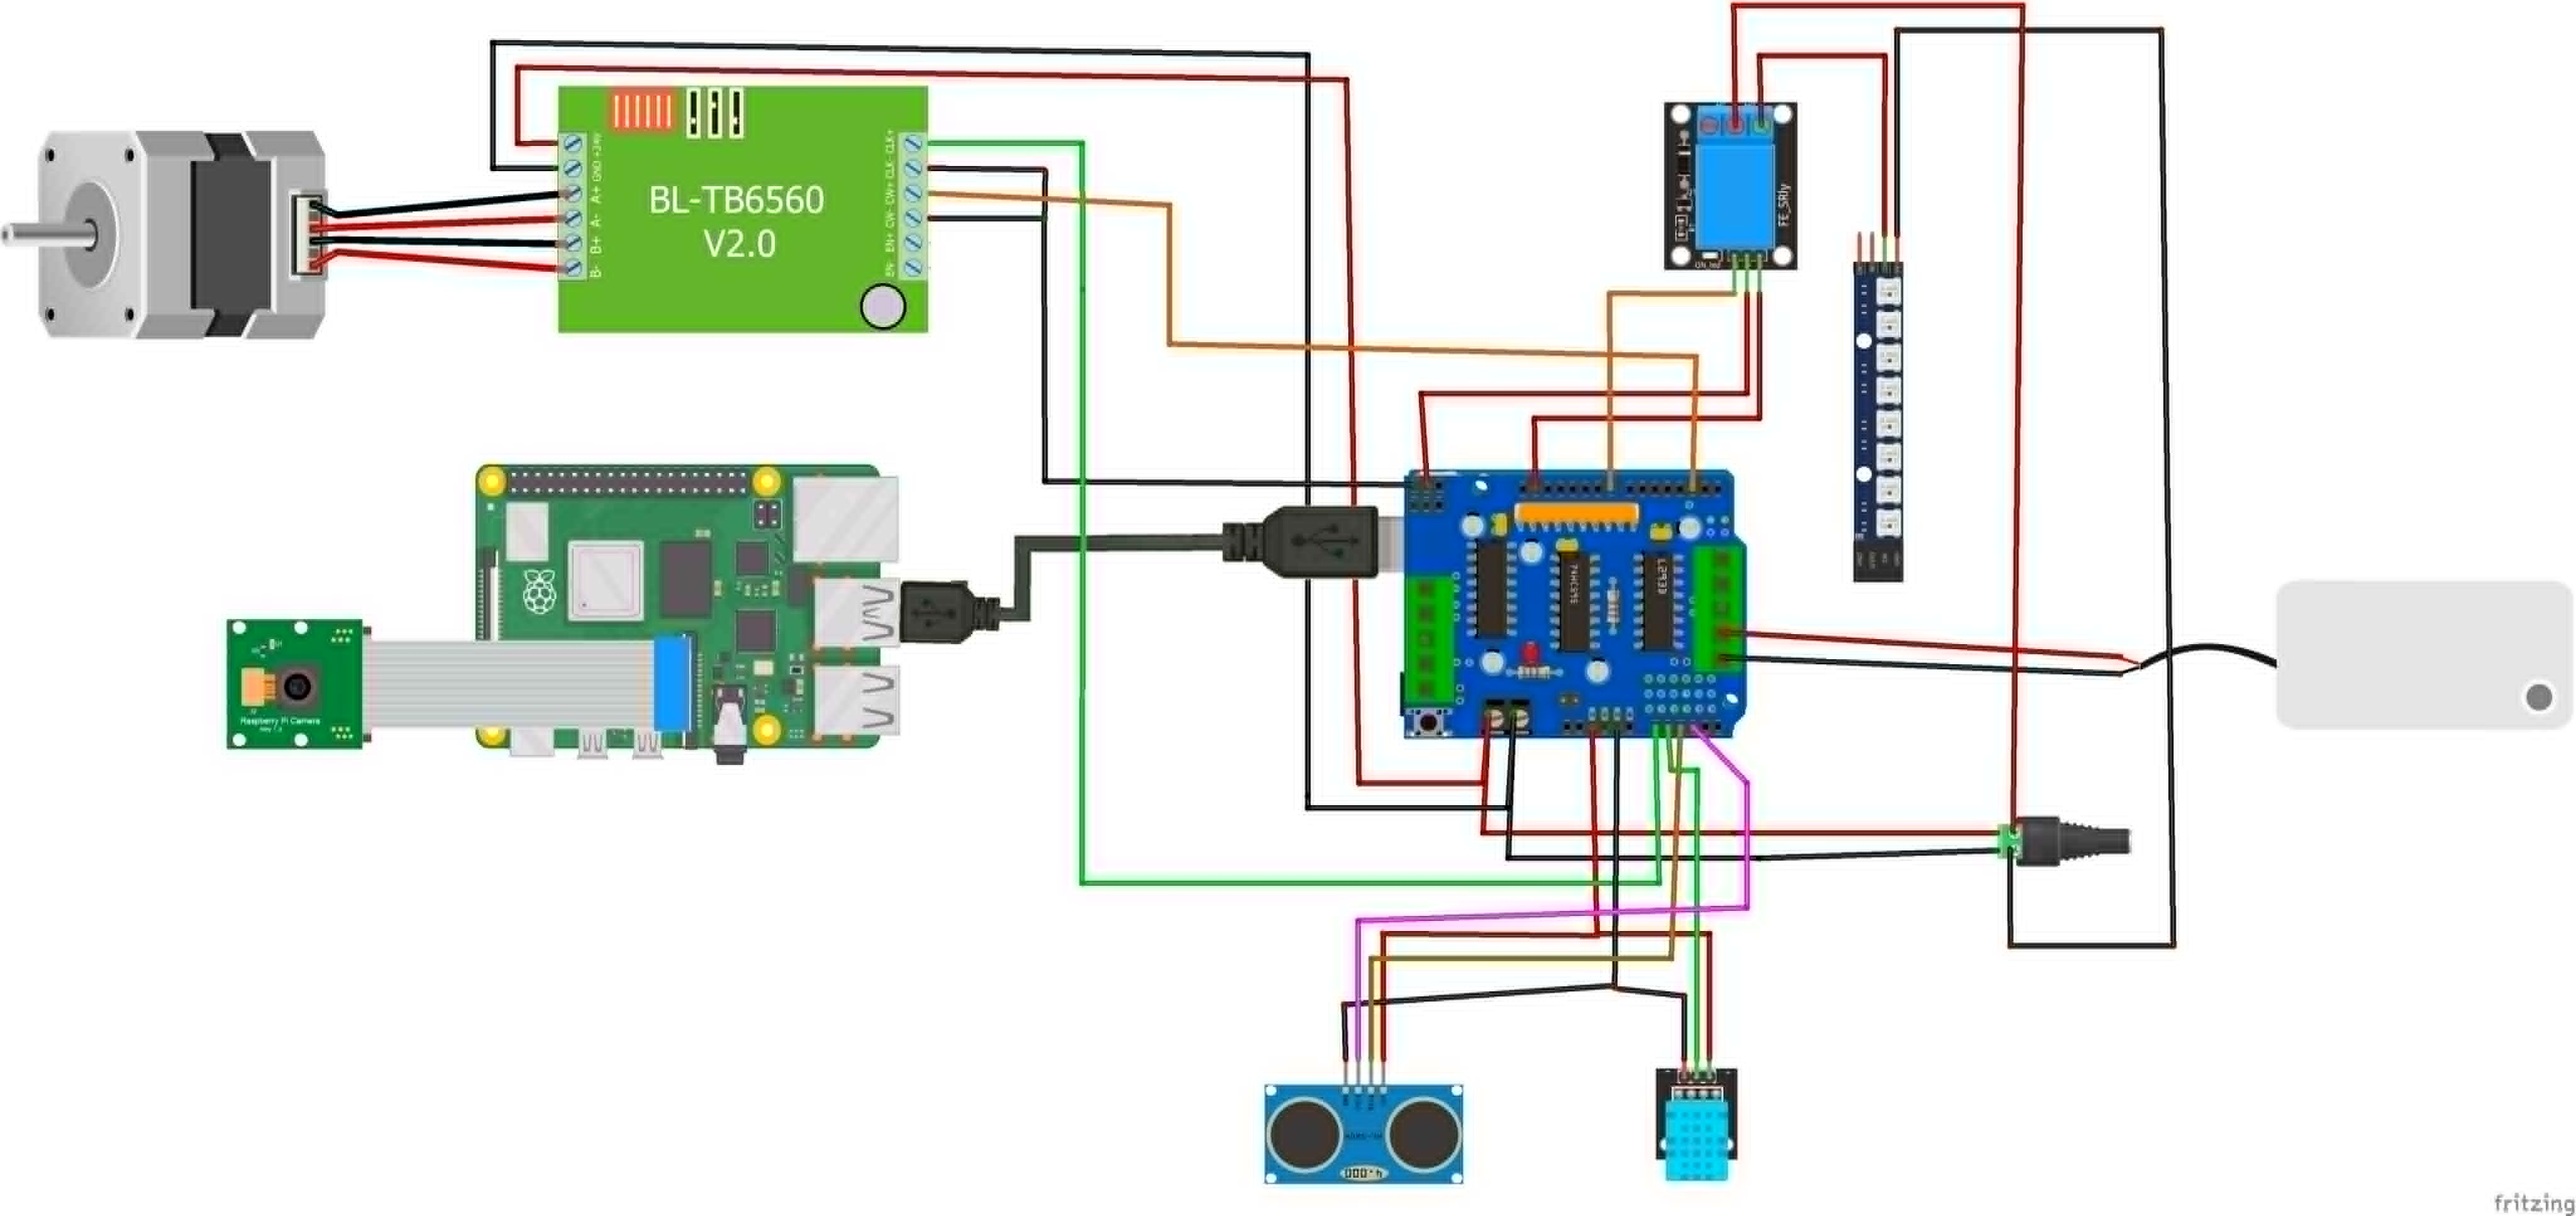
\includegraphics[width=0.7\linewidth]{public/cablage}
	\caption{Schéma détaillé du câblage des capteurs et actionneurs avec le microcontrôleur}
	\label{fig:cablage}
\end{figure}

La figure~\ref{fig:cablage} vient ainsi compléter la figure~\ref{fig:archi_iot} en apportant une vue détaillée de l’implémentation matérielle, depuis l’architecture globale jusqu’au niveau des connexions physiques.

\subsubsection*{Architecture logicielle embarquée}
La couche embarquée n'est pas figée : le logiciel exécuté sur le contrôleur est entièrement \textbf{versionné et mis à jour à distance} (voir la section~\ref{subsec:ota_thingsboard} consacrée à l'OTA). Sur le plan logiciel, le système embarqué se décompose en \textbf{deux ensembles complémentaires} :

\begin{itemize}
	\item \textbf{Le composant principal (« Main ») :} il regroupe le \textit{logiciel} déployé sur le Raspberry~Pi~4 et le \textit{micrologiciel} (\textit{firmware}) déployé sur l'Arduino. Le logiciel constitue le cœur applicatif du contrôleur : il établit et maintient la connexion MQTT avec le backend, dialogue avec le module d'intelligence artificielle et traduit les consignes reçues en commandes transmises au micrologiciel. Le micrologiciel, quant à lui, exécute de manière déterministe les tâches matérielles de proximité (acquisition des capteurs et pilotage des actionneurs).
	\item \textbf{Le service ThingsBoard (agent de déploiement) :} il s'agit d'un service autonome dont l'unique vocation est d'\textit{installer, surveiller et mettre à jour} le composant principal (logiciel et micrologiciel). Il assure l'enregistrement du contrôleur auprès de la plateforme ThingsBoard et orchestre l'application des mises à jour distantes (OTA), garantissant ainsi que la serre exécute toujours la dernière version validée du logiciel.
\end{itemize}
\begin{figure}[!htbp]
	\centering
	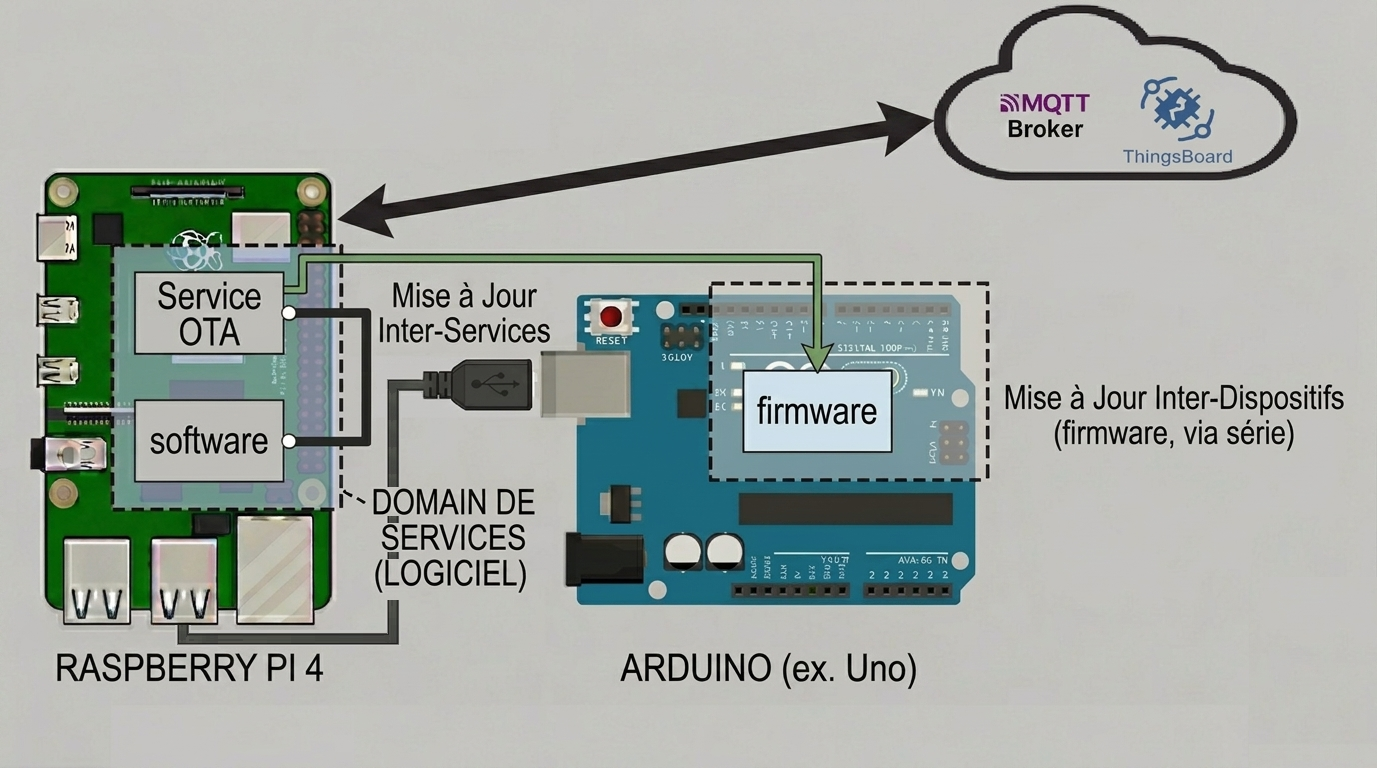
\includegraphics[width=0.7\linewidth]{public/relationLogEmbeded}
	\caption{Relation entre le composant principal et le service de déploiement ThingsBoard}
	\label{fig:relation_log_embedded}
\end{figure}
\paragraph{Architecture au sein du Raspberry Pi 4}
Le Raspberry Pi 4 constitue l'unité de coordination du système embarqué. Il héberge le logiciel principal (services de supervision, de communication et d'orchestration des traitements locaux) ainsi que l'agent de déploiement ThingsBoard. Son rôle principal est de centraliser les échanges avec le backend via MQTT, de dialoguer avec le module IA et de piloter la logique globale de la serre en relayant les commandes vers l'Arduino.

\begin{figure}[!htbp]
	\centering
	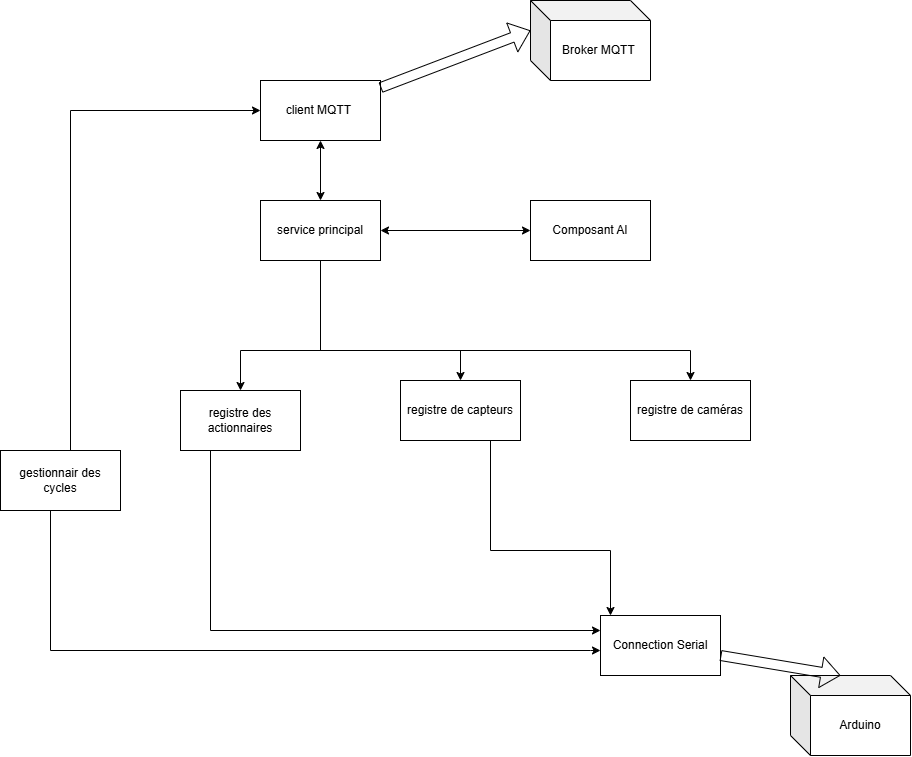
\includegraphics[width=0.9\linewidth]{public/raspiArchiDiagFR.png}
	\caption{Architecture logicielle embarquée au sein du système}
	\label{fig:embeededsoft}
\end{figure}

\paragraph{Architecture au sein de l'Arduino}
L'Arduino est dédié à l'exécution déterministe des tâches matérielles de proximité. Il prend en charge la lecture périodique des capteurs, la commande des actionneurs et l'application des consignes envoyées par le Raspberry Pi 4 via une liaison série. Cette séparation permet de conserver un comportement stable pour les opérations temps réel tout en réservant au Raspberry Pi les fonctions de communication.

L'implémentation du firmware embarqué a été confrontée à une contrainte importante liée aux ressources matérielles limitées de l'Arduino Uno, qui ne dispose que de 2 Ko de mémoire SRAM. Dans ce contexte, une architecture orientée objet classique basée sur l'héritage, le polymorphisme et l'instanciation de nombreuses classes aurait entraîné une consommation mémoire significative dès le démarrage du système.

Afin de garantir la compatibilité avec les ressources disponibles tout en conservant une architecture modulaire et extensible, une approche alternative a été adoptée. Celle-ci repose sur l'utilisation de structures légères associées à des pointeurs de fonctions permettant de représenter les différents périphériques de manière générique sans recourir à une hiérarchie complexe de classes.

Cette stratégie présente plusieurs avantages. D'une part, elle réduit considérablement l'occupation mémoire en supprimant les surcoûts associés aux mécanismes orientés objet traditionnels. D'autre part, elle permet d'ajouter de nouveaux périphériques en définissant uniquement les données spécifiques et les opérations nécessaires à leur fonctionnement. Enfin, l'ensemble des équipements peut être géré à travers une interface commune tout en conservant une empreinte mémoire compatible avec les contraintes du microcontrôleur.

Cette optimisation a permis d'intégrer simultanément plusieurs capteurs et actionneurs au sein du même firmware tout en préservant suffisamment de mémoire pour les buffers de communication série, les bibliothèques matérielles et les traitements temps réel nécessaires au fonctionnement de la serre intelligente.


Cette répartition des responsabilités garantit une architecture plus robuste : le Raspberry Pi 4 concentre les services applicatifs et intelligents, tandis que l'Arduino reste responsable du contrôle matériel de bas niveau.
\subsubsection*{Structure des messages série (Raspberry Pi \texorpdfstring{$\leftrightarrow$}{<->} Arduino)}
La communication entre le Raspberry Pi 4 et l'Arduino repose sur une liaison série UART utilisant un protocole de messages textuels structurés. Cette approche permet de simplifier le décodage des commandes tout en garantissant la lisibilité et la maintenabilité des échanges.

Les commandes envoyées par le Raspberry Pi respectent le format général suivant :


\texttt{<nom\_equipement>:<action>:<parametre\_1>:<parametre\_2>:...}


où :

\begin{itemize}
	\item \texttt{<nom\_equipement>} identifie le périphérique concerné ;
	\item \texttt{} représente l'opération à exécuter ;
	\item \texttt{<parametre\_i>} correspond aux paramètres associés à cette opération.
\end{itemize}

Par exemple, la commande :


\texttt{dc1:SPEED:200}


ordonne au moteur \texttt{dc1} de fonctionner à une vitesse de \texttt{200}.

Les réponses générées par l'Arduino utilisent quant à elles l'un des formats suivants :


\texttt{OK:value}


ou


\texttt{ERR:message}


Le premier indique l'exécution correcte de la commande tandis que le second signale une erreur détectée lors du traitement , par example : \texttt{OK:done} , \texttt{ERR:bad\_action}

\subsubsection*{Sécurité des communications IoT (MQTTS et TLS)}
Étant donné la nature critique des commandes transitant entre le Backend et la serre (ex: pilotage des pompes et vannes d'irrigation), la sécurité réseau est une composante structurelle de l'architecture. Toutes les communications télémétriques entre l'unité \textit{Edge} (Raspberry Pi 4) et le broker Mosquitto sont encapsulées dans un tunnel crypté utilisant le protocole \textbf{MQTTS} (MQTT sur TLS 1.2+). L'authentification mutuelle est assurée par l'échange de certificats X.509 et de clés asymétriques, prévenant ainsi toute attaque de type \textit{Man-in-the-Middle} (MitM) ou l'injection de fausses commandes matérielles. De plus, aucun secret critique (mot de passe base de données, clé d'API Gemini) n'est stocké en clair sur le dispositif physique local.

\subsubsection*{Mode Autonome (Architecture Offline-First)}
Conçu selon le paradigme \textit{Offline-First}, le contrôleur conserve une autonomie de fonctionnement complète en cas de coupure réseau : les cycles d'irrigation, d'éclairage et de ventilation sont maintenus localement à partir de la dernière configuration valide, tandis que les relevés non transmis sont temporisés dans un tampon local (SQLite) avant d'être resynchronisés avec le backend dès le rétablissement de la connexion.

\subsection{Le mécanisme d'attention et les Transformers}
Introduit pour le traitement automatique des langues~\cite{vaswani2017attention}, le mécanisme d'\textbf{auto-attention} permet à chaque élément d'une séquence d'interagir directement avec tous les autres, contrairement aux CNN qui ont une vision locale. Cette capacité à capturer des dépendances à longue distance est particulièrement utile en agriculture pour relier des symptômes distants sur une même plante. Les Transformers sont gourmands en données et en calcul, mais des variantes comme le \textbf{Swin Transformer}~\cite{liu2021swin} réduisent la complexité en limitant l'attention à des fenêtres locales.

\subsection{Grands modèles de langage (LLM)}
Les LLM (GPT, Gemini, etc.) sont des Transformers de type décodeur entraînés sur des masses de texte. Ils excellent en raisonnement et en génération de texte, mais sont \textbf{aveugles} : ils ne peuvent analyser une image. Pour le diagnostic agricole, ils doivent être combinés à un encodeur visuel.

\subsection{Modèles vision-langage (VLM)}
Un VLM associe trois composants : (1) un encodeur visuel (souvent un Vision Transformer), (2) un module d'alignement (projecteur ou Q-Former), (3) un LLM qui reçoit à la fois les tokens visuels et la question textuelle. Le tableau~\ref{tab:vlm_models} résume l'évolution récente.

\begin{table}[htbp]
	\centering
	\small
	\begin{tabularx}{\textwidth}{|l|c|Y|}
		\hline
		\rowcolor[HTML]{2C3E50}
		\textcolor{white}{\textbf{Modèle}} & \textcolor{white}{\textbf{Année}} & \textcolor{white}{\textbf{Innovation}} \\ \hline
		CLIP~\cite{radford2021learning} & 2021 & Apprentissage contrastif image-texte. \\
		BLIP-2~\cite{li2023blip2} & 2023 & Q-Former pour aligner vision et langage. \\
		LLaVA~\cite{liu2023llava} & 2023 & Projection linéaire + réglage par instructions. \\
		InstructBLIP~\cite{dai2023instructblip} & 2023 & Conditionnement du Q-Former par la question. \\
		\textbf{PaliGemma}~\cite{beyer2024paligemma} & 2024 & Architecture unifiée SigLIP + Gemma 2B. \\ \hline
	\end{tabularx}
	\caption{Évolution des modèles vision-langage}
	\label{tab:vlm_models}
\end{table}

La \textbf{question-réponse visuelle (VQA)} concrétise l'usage des VLM : l'utilisateur interroge le système en langage naturel, et le modèle répond en décrivant les symptômes (figure~\ref{fig:vqa-architecture}). Les VQA offrent une interaction guidée et une explicabilité, mais souffrent encore d'hallucinations, d'une forte dépendance au cloud, et d'une sensibilité aux conditions de prise de vue.

\begin{figure}[tbph]
	\centering
	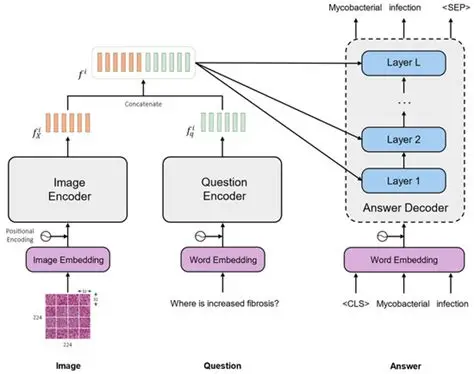
\includegraphics[width=0.7\linewidth]{public/vqa-architecture}
	\caption{Architecture fonctionnelle d'un système VQA.}
	\label{fig:vqa-architecture}
\end{figure}

\begin{figure}[tbph]
	\centering
	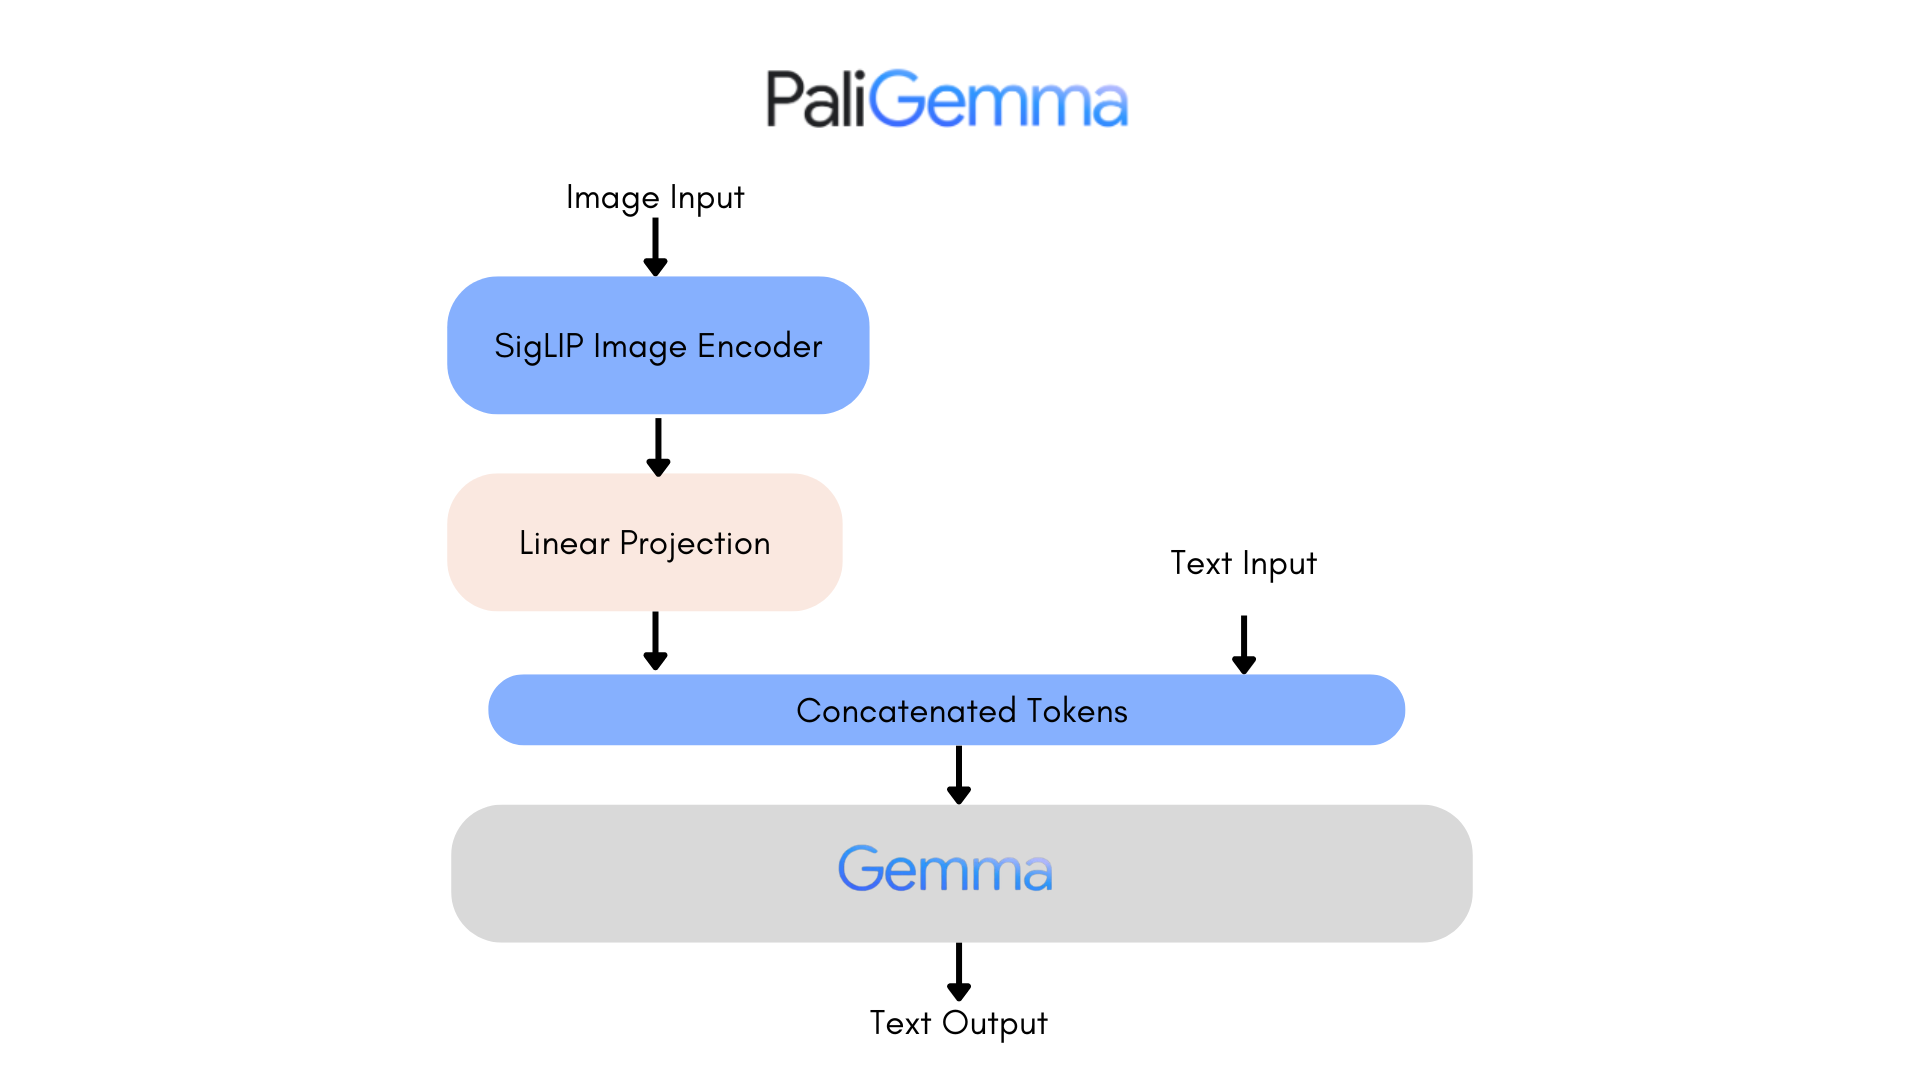
\includegraphics[width=0.7\linewidth]{public/paligemma_arch}
	\caption{Architecture de PaliGemma (SigLIP + Gemma).}
	\label{fig:paligemmaarch}
\end{figure}

% ============================================================

% ============================================================
\section{Apprentissage adaptatif et dynamique}
\label{sec:adaptive_dynamic}

L’agriculture de précision impose des modèles capables de s’adapter à des conditions changeantes (nouvelles maladies, variétés de plantes, environnements) tout en restant robustes et explicables. Cette section explore les techniques d’apprentissage qui permettent cette adaptabilité : les méthodes ensemblistes, l’apprentissage avec peu d’exemples (few-shot) et avec zéro exemple (zero-shot), ainsi que la sélection dynamique d’ensemble.

\subsection{Apprentissage par ensembles}
Les méthodes d’ensemble classiques, comme le \textit{bagging} (forêts aléatoires) ou le \textit{boosting} (AdaBoost, XGBoost), combinent plusieurs classifieurs pour réduire la variance et le biais. Appliquées aux réseaux de neurones, elles améliorent la robustesse : un ensemble de CNN peut surpasser n’importe lequel de ses membres pris isolément~\cite{dietterich2000ensemble}. Cependant, ces approches restent \textbf{statiques} : la combinaison des modèles est figée une fois l’entraînement terminé. Or, un modèle peut exceller sur certaines régions de l’espace des caractéristiques et être médiocre sur d’autres.

\subsection{Apprentissage avec peu d’exemples (few-shot)}
En environnement agricole réel, il est fréquent de devoir identifier une nouvelle maladie ou une variété végétale pour laquelle on ne dispose que de très peu d’images (parfois moins d’une dizaine). L’\textbf{apprentissage avec peu d’exemples} (few-shot learning) répond à ce besoin. Le \textbf{méta-apprentissage} (\textit{learning to learn}) en est une approche phare : l’algorithme MAML~\cite{finn2017model} apprend une initialisation des paramètres telle qu’une ou deux étapes de descente de gradient suffisent à adapter le modèle à une nouvelle tâche avec très peu de données. Cette capacité est cruciale pour un système comme HydroNova, qui doit pouvoir évoluer avec l’apparition de nouveaux pathogènes. D'autres approches comme \textit{Prototypical Networks}~\cite{snell2017prototypical} ou \textit{Relation Networks}~\cite{sung2018learning} sont également utilisées en agriculture~\cite{arguello2020few}.

\subsection{Apprentissage avec zéro exemple (zero-shot)}
Dans certains cas, aucune image de la nouvelle maladie n’est disponible au moment de l’entraînement. L’\textbf{apprentissage avec zéro exemple} (zero-shot learning) exploite des descriptions sémantiques (textuelles) des classes cibles. Les modèles vision-langage (VLM) comme CLIP~\cite{radford2021learning} ou PaliGemma sont naturellement adaptés au zero-shot : ils comparent l’image à une description textuelle de la maladie (par exemple, \textit{« taches brunes entourées d’un halo jaune sur feuilles de tomate »}) sans avoir jamais vu d’exemple visuel de cette pathologie. Cette approche est particulièrement pertinente pour les émergences phytosanitaires rapides~\cite{li2020zero}.

\subsection{Sélection dynamique d’ensemble (DES)}
Pour pallier le caractère statique des ensembles classiques, la \textbf{sélection dynamique d’ensemble} (DES) choisit, pour chaque image à classer, les modèles les plus compétents localement. Le framework \textbf{META-DES}~\cite{cruz2018meta} procède ainsi :
\begin{enumerate}
	\item Définition d’un voisinage de l’image cible (ses plus proches voisins dans un ensemble de validation).
	\item Extraction de \textit{méta-caractéristiques} pour chaque modèle candidat (précision locale, niveau de confiance, etc.).
	\item Prédiction par un méta-classifieur de la compétence du modèle pour cette image.
	\item Vote pondéré des seuls modèles jugés compétents.
\end{enumerate}
Cette approche améliore significativement la précision et la robustesse, particulièrement utile en milieu agricole où les conditions d’acquisition (éclairage, angle, chevauchement) varient fortement. Des travaux récents l'appliquent au diagnostic de maladies des plantes~\cite{zhang2020dynamic}.

\subsection{Pertinence dans le contexte agricole}
L’apprentissage adaptatif et dynamique répond à plusieurs contraintes du projet HydroNova :
\begin{itemize}
	\item \textbf{Évolutivité} : l’apparition de nouvelles maladies ou de nouvelles variétés de plantes peut être prise en compte via le few-shot ou le zero-shot, sans réentraînement complet.
	\item \textbf{Robustesse aux variations} : la sélection dynamique d’ensemble permet de s’adapter localement à des conditions de terrain changeantes.
	\item \textbf{Hybridation Edge/Cloud} : le few-shot et le zero-shot peuvent être déployés en cloud (via VLM), tandis que la sélection dynamique d’ensemble peut être embarquée sur le Raspberry Pi pour une inférence rapide hors-ligne.
\end{itemize}
Ces techniques complètent ainsi naturellement l’architecture hybride proposée : le module embarqué repose sur un ensemble dynamique de CNN (DES), tandis que le module cloud exploite un VLM capable de zero-shot et de few-shot.

% ============================================================
\section{Synthèse critique et positionnement}
\label{sec:synthese}

Le tableau~\ref{tab:synthese} compare les différentes familles de modèles selon des critères opérationnels.

\begin{table}[htbp]
	\centering
	\small
	\begin{tabularx}{\textwidth}{|l|X|X|c|c|}
		\hline
		\rowcolor[HTML]{2C3E50}
		\textcolor{white}{\textbf{Approche}} & \textcolor{white}{\textbf{Apports}} & \textcolor{white}{\textbf{Limites}} & \textcolor{white}{\textbf{Offline}} & \textcolor{white}{\textbf{Explicabilité}} \\ \hline
		CNN classiques & Efficaces, légers & Fragiles, boîtes noires & Oui & Faible \\
		Ensembles de CNN & Robustesse & Complexité & Oui & Faible/Moyenne \\
		Vision Transformers & Modélisation globale & Gourmands & Partiel & Moyenne \\
		LLM & Raisonnement, texte & Aveugles & Non & Élevée \\
		VLM / VQA & Multimodal, explicatif & Hallucinations, dépendance cloud & Non & Élevée \\
		Few-shot / Zero-shot & Adaptabilité rapide & Nécessite un pré-entraînement adapté & Partiel & Moyenne/Élevée \\
		DES (sélection dynamique) & Robustesse locale & Coût de calcul supplémentaire & Oui & Moyenne \\ \hline
	\end{tabularx}
	\caption{Synthèse comparative des paradigmes d'IA pour le diagnostic agricole}
	\label{tab:synthese}
\end{table}

Aucune approche unique ne satisfait toutes les contraintes du projet HydroNova : besoin d'un fonctionnement hors-ligne (serres isolées), de robustesse aux conditions réelles, d'évolutivité face à de nouvelles maladies, et d'explicabilité pour l'utilisateur.

C'est pourquoi nous proposons une \textbf{architecture hybride} articulant deux branches complémentaires :

\begin{itemize}
	\item Une branche \textbf{Edge} (embarquée sur Raspberry Pi) basée sur un ensemble dynamique de CNN (META-DES) pour une classification robuste, rapide et hors-ligne.
	\item Une branche \textbf{Cloud} exploitant un VLM (PaliGemma) pour l'assistance interactive, la génération d'explications, les cas ambigus, ainsi que l'adaptation en cas d'absence d'exemples.
\end{itemize}

Cette hybridation permet de concilier performance, résilience, adaptabilité et richesse sémantique.

% ============================================================
\section*{Conclusion}
\addcontentsline{toc}{section}{Conclusion}

Ce chapitre a présenté un panorama des principales architectures d'intelligence artificielle pour l'agriculture : CNN, Transformers, VLM, ainsi que les techniques d'apprentissage adaptatif et dynamique (ensembles, few-shot, zero-shot, sélection dynamique). L'analyse montre qu'aucun modèle isolé n'est suffisant, ce qui justifie l'approche hybride d'HydroNova. Le chapitre suivant détaille l'analyse des besoins et la spécification fonctionnelle du système.